\section{Electric field sensing}
Electricity, as a force has been known for millennia. However, it has not bloomed until the 18th century, when it was turned from a curiosity into a science over the course of the next 200 years. In 1858 famous chemist and physicist Michael Faraday noted:
\begin{quote}
Electricity is often called wonderful, beautiful; but it is so only in common with the other forces of nature. The beauty of electricity or of any other force is not that the power is mysterious, and unexpected, touching every sense at unawares in turn, but that it is under law, and that the taught intellect can even now govern it largely. \cite{jones1870life}
\end{quote}
One of those laws is that different electric charges apply either a repelling or attracting force to each other. For any point in space these forces have a distinct direction and magnitude. The resulting collection of force vectors is called the electric field. Conductive objects that are present in this area modify the properties of the field. Electric field sensing enables measuring field properties at a certain point in space. Using continuous monitoring it is possible to gather information about conductive objects passing through the field by associating measured disturbances to properties of the object. It is possible to gather a multitude of different information about a project. In this section I will give an overview of the physical background, different measurement modes and how to process data acquired by digital sensors. This section is extended from the version presented in \cite{braun2014capjaise}.
\subsection{Physical properties}
A complete overview about the electrostatic principles of capacitive proximity sensing can be found in the book by Baxter \cite{Baxter1996}, chapters 2 and 6. In the following paragraphs I will give a very brief introduction to this topic.
\begin{figure}[h]
\centering
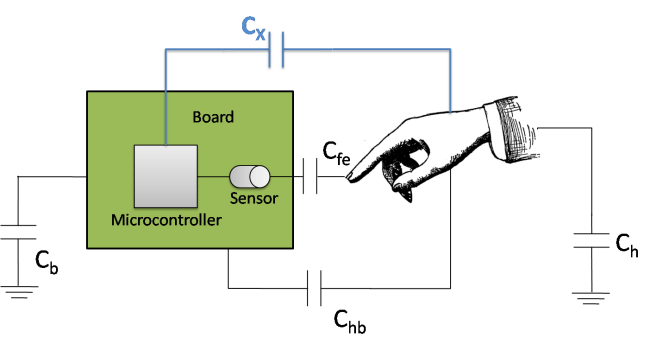
\includegraphics[width=0.4\textwidth]{images/cap_blackbox.png}
\caption{Black box setup of a capacitive proximity sensor}
\label{fig:cap_blackbox}
\end{figure}
The basic setup of a typically used sensor is shown in Figure \ref{fig:cap_blackbox}. The proximity capacitance \(C_{x}\) can be determined using a combination of serial and parallel circuits of capacitors, resulting in the following equation:
\begin{equation}
C_{x}=\left(\left(C_{hb}+\frac{C_{h}C_{b}}{C_{h}+C_{b}}\right)^{-1}\frac{1}{C_{fe}}\right)^{-1}
\end{equation}
Additionally there are parasitic capacitance components, i.e. disturbing capacitance values within the system. It can be caused by a variety of different sources. These include:
\begin{itemize}
\item Capacitance of the sensing electrode 
\item Capacitance between sensing electrode and ground plane
\item Intercapacitance between neighboring traces on the board
\end{itemize}
Looking at a typical system, the combined parasitic capacitances \(C_{par}\) amounts to values approximately between \(10pF\) and \(300pF\) and is therefore considerably larger than the value of the proximity capacitance \(Cx\), being between \(0.1pF\) and \(10pF\). The total capacitance sensed is the sum of parasitic and proximity components. 
\begin{equation}
C_{S}=C_{X}+C_{par}
\end{equation}

While this parasitic capacitance can be orders of magnitudes higher than the capacitance that is to be measured, it is typically static in a given system. There are some disturbing factors and changes over time that have to be accounted for. Those will be further discussed in the processing sections. This static value can be determined periodically and filtered out of the resulting value, allowing to get a suitable measurement. 
\begin{figure}[h]
\centering
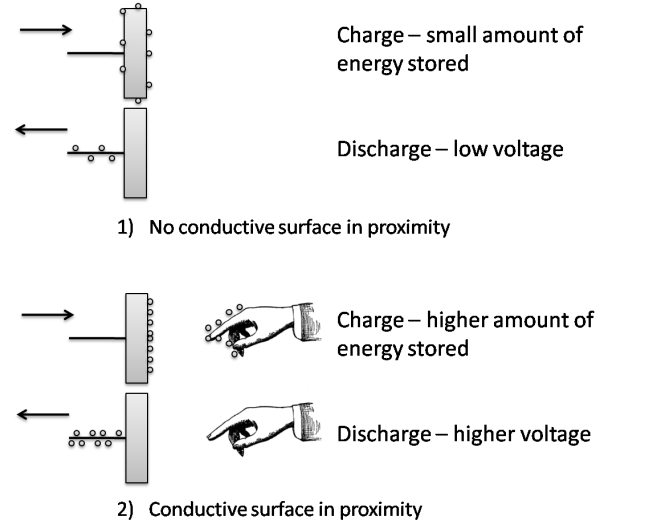
\includegraphics[width=0.4\textwidth]{images/cap_procedure.png}
\caption{Capacitive sensing procedure}
\label{fig:cap_procedure}
\end{figure} 
In electric field sensing the idea is to measure the distance of objects from the sensing electrode. Thus it is necessary to discuss how the capacitance of common objects approaching the sensor can be estimated. Any object exhibits capacitance in respect to infinity. Surveying simple geometric shapes this capacitance is analytically determinable, e.g.:
\begin{equation}
C=8\epsilon_{0}r_{Disk}
\end{equation}
\begin{equation}
C=4\pi\epsilon_{0}r_{Sphere}
\end{equation}

\(\epsilon_{0}\) is the vacuum permittivity and \(r\) the respective radius. This free space capacitance is increasing as soon as another object is approaching, caused by the capacitance of this second object, resulting in mutual capacitance, i.e. the resulting capacitive properties between a sending and a receiving object that are close to each other. Looking at generic formulas, determining capacitance between parallel plates this behavior can be described analytically.
\begin{align}
C&=\frac{Q}{V} & C&=\epsilon_{0}\epsilon_{r}\frac{A}{d}
\end{align}
The capacitance is directly proportional to the plate area \(A\) and inversely proportional to the distance d between the plates, with \(\epsilon_{r}\) being the relative static permittivity of the dielectric between the plates. Sensor electronics are grounded with the body acting as ground itself. The sensor plate is continuously charged using a constant voltage \(V\). A higher capacitance allows the system to hold a larger charge. If the system is connected to the ground, the sensor capacitor is discharged through a resistor. The resulting voltage is depending on the available charge, shown in the equation above. Furthermore the required time to discharge the capacitor is increased. This process is symbolized in Figure \ref{fig:cap_procedure}.

\subsection{Proximity sensing versus touch sensing}
\begin{figure}[h]
\centering
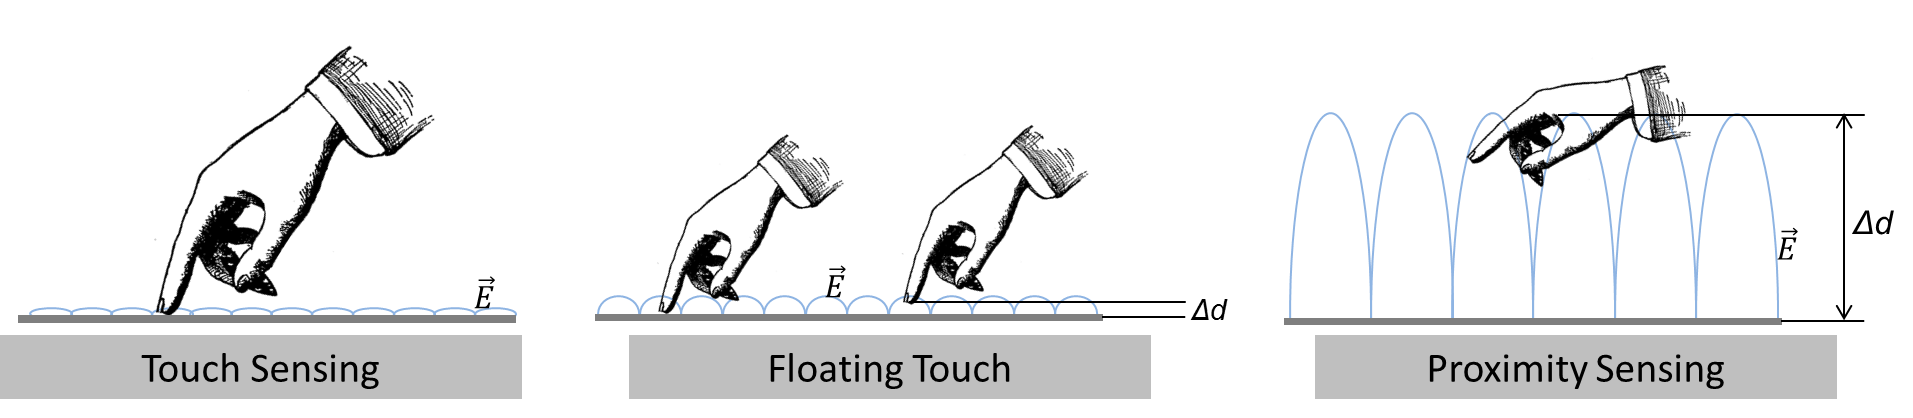
\includegraphics[width=1.0\textwidth]{images/cap_projected_sensing_methods.png}
\caption{Different projected capacitive sensing methods based on distance}
\label{fig:cap_proj_sensing_methods}
\end{figure} 
The most ubiquitous usage of capacitive sensing technology is touch screens. As the trend went from pen-controlled mobile systems to finger controlled devices with the first iPhone in 2007, projected capacitance touch is the most prevalent technology for touch screens. It uses various layers of transparent electrodes or very thin wires to measure the mutual capacitance as objects enter the detection area \cite{Barrett2010}. The commercially available devices have gained additional abilities over the last few years, leading to the development of "floating touch" systems that are able to track fingers in gloves, or fingers that are hovering above the surface \cite{Cypress2012, Nokia2012}. Applications are the usage of mobile devices in cold outdoor temperatures or additional navigation features based on the hovering fingers. In consequence it is possible to distinguish the three different projected capacitive sensing methods shown in Figure \ref{fig:cap_proj_sensing_methods}:
\begin{itemize}
\item Touch sensing - densely distributed sensors are tuned to project a weak electric field in order to detect one or more objects touching the interactive surface. The sensors have to be close to the surface.
\item Floating touch - densely distributed high-sensitivity sensors are able to detect both touches and very near objects (\(<2cm\)) to enable usage using protective gear or additional navigation feature. The sensors have to be close to the surface.
\item Proximity sensing - sparsely distributed sensors create a stronger electric field that propagates into space in order to detect larger objects, such as hands, that are in proximity of the interactive surface. Achievable distances exceed 30 centimeters and the sensors may be applied below thick non-conductive material.
\end{itemize}
\subsection{Measuring modes}
\begin{figure} [h]
\centering
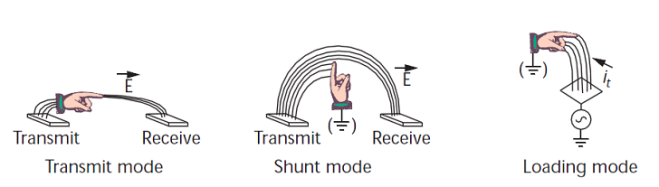
\includegraphics[width=0.8\textwidth]{images/cap_sensing_modes.png} 
\caption{Three measurement modes for capacitive proximity sensing \cite{Smith1996a}}
\label{fig:cap_sensing_modes}
\end{figure}
A classic work in the field of capacitive proximity sensing that will be referenced occasionally in this work is "Electric Field Imaging" by Joshua Smith \cite{smith1999thesis}. One contribution was the introduction of different measurement modes that can be distinguished in capacitive sensing. They are shown in Figure \ref{fig:cap_sensing_modes}. 

Transmit mode is using a transmitting electrode that is coupled to a conductive object - in case of human-machine interaction applications, typically the human body. The properties of an electric field generated with respect to a receiving electrode will therefore be dependent on the distance of this body, thus extending the achievable range.

Shunt mode similarly uses both a receiving and transmitting electrode generating a static field. However, there is no body coupled and any conductive object will ground the field, thus reducing the energy stored, which is measured. This setup is able to work with various transmitters on a single receiver, enabling a higher amount of virtual sensors using limited hardware. 

The third measurement mode is called loading mode. An oscillating field is induced on a single electrode measuring the capacitance relative to the environment. Any approaching grounded object results in an increased capacitance that is measured periodically.
\subsection{Materials and geometry}
Two major factors that have to be considered when designing an application based on capacitive sensors are the materials and geometry of the electrodes performing the measurements. The material of the electrode should be picked according to the desired application, i.e. if the interaction device has a flexible surface, conductive thread could be used, if it is solid and opaque, the application of solid metal electrodes is viable. Additionally there are other options for transparent materials. 

While we traditionally associate solid metals to antennas and electrodes this view can no longer be upheld. Transparent conductive layers have been in use for decades now, e.g. in car windows or solar technology. They typically rely on metal oxide layers, polymer layers or in recent years carbon nanotubes \cite{Moon2005}. The most common technology for usage in displays is projected capacitive touch that uses a multi-layer design of insulated ITO electrodes that are able to detect the movement of several objects close to the surface \cite{Barrett2010}. However, they are typically tuned to allow operation within a small distance of 1cm or less. However, they are typically tuned to allow operation within a small distance of 1cm or less. 

In the scope of his Master's thesis Yannick Berghöfer evaluated different types of electrode materials in terms of their spatial resolution at different distances between object and electrode. The results were included in the following paper of our group \cite{grosse2013opencapsense}. The focus was to establish how the different materials perform at larger distances. The benchmarked materials included both ITO and PEDOT:PSS. The first is a thin layer of indium-titanium-oxide, a highly conductive metal layer that possesses good optical properties. PEDOT:PSS is a conductive polymer that has a lower conductivity and slightly less appealing optical properties. In conclusion it could be estalbished that while copper has still the most favorable properties, at least ITO can be considered a suitable alternative in applications that require optical transparency. An overview of the achievable spatial resolutions of the different materials and and electrode sizes is given in Figure \ref{fig:cap_spatial_resolution}.  The spatial resolution is a measure that describes the expected precision of the measurement based on taking a time series of multiple samples and determining the mean distance and standard deviation \cite{grosse2013opencapsense}.
\begin{figure} [h]
\centering
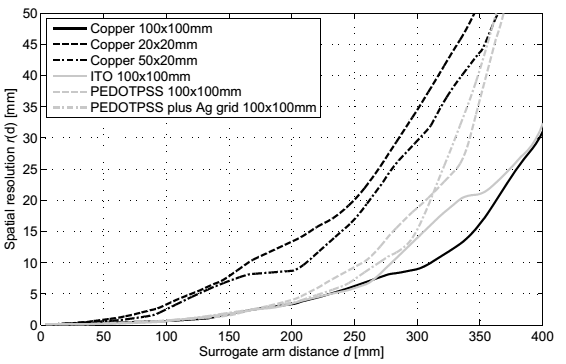
\includegraphics[width=0.6\textwidth]{images/cap_spatial_resolution.png} 
\caption{Spatial resolution of different materials at various distances \cite{grosse2013opencapsense}}
\label{fig:cap_spatial_resolution}
\end{figure}

The most common technology for usage in displays is projected capacitive touch that uses a multi-layer design of insulated ITO electrodes that are able to detect the movement of several objects close to the surface \cite{Barrett2010}. However, they are typically tuned to allow operation within a small distance of 1cm or less. 
Another area that is strongly influenced by the intended application is the geometry, whereas the electrode is considered the part of the electronics directly attached to the measurement circuit. This may range from simple straight wires or plate electrodes to complex optimized multidimensional structures specifically designed for a single task. Even though it is aimed at touch or near-proximity sensing I will give a short overview of  multi-layer designs for touch screens that have been reviewed by Barrett and Omote \cite{BarrettScreen}. They are designed to measure mutual capacitance. If a sensible excitation and measuring process is used, multiple nearby objects may be reliably detected. 
\begin{figure} [h]
\centering
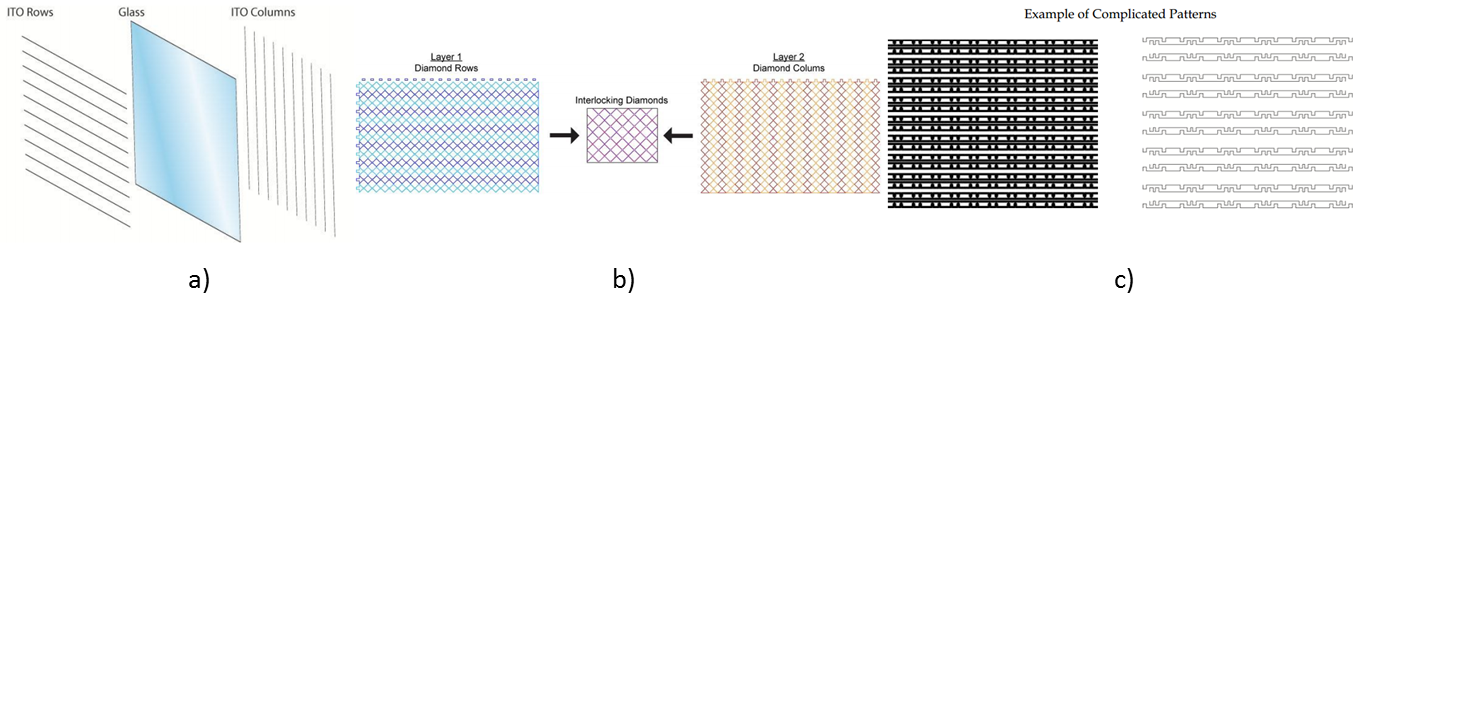
\includegraphics[width=0.8\textwidth]{images/ito_multilayer} 
\caption{Examples of multilayer layouts for touch screens - grid (a), interlocking diamonds (b) and  trademarked complex patterns (c) \cite{BarrettScreen}}
\label{fig:ito_multilayer}
\end{figure}
A simple example is two layers of perpendicular straight line electrodes - used by the first iPhone (Figure \ref{fig:ito_multilayer} - a). Another example uses an interlocking diamond shape \cite{Dietz2001a} to create a good spatial coverage (Figure \ref{fig:ito_multilayer} - b). Finally, there are numerous other complex patterns that are often trademarked by the companies that have developed the respective controller. One example is given in (Figure \ref{fig:ito_multilayer} - c). 

Capacitive proximity sensing applications are typically less concerned about intricate designs, but instead use varying electrode sizes and placement over a larger area. As previously mentioned the purpose of capacitive proximity sensing is the detection of objects and their properties. There are numerous factors that can influence the geometrical layout, but they can be abstracted into the following categories:
\begin{itemize}
\item	Number of objects
\item	Object size
\item	Desired spatial resolution
\end{itemize}
Going back to our example of touch screens, there are small objects, a higher number of those (usually up to 10) and require a high spatial resolution to select small items on the screen. The result is a fine multilayer grid, using mutual capacitance to simplify multi-object recognition, fine electrode spacing to achieve a high spatial resolution and thin wires or transparent electrodes to guarantee good optical properties. A similar rationale can be applied to other applications. Taking the smart couch created by Tobias Große-Puppendahl, Alexander Marinc and myself, the aim is to detect the presence and posture of one or more persons on a couch \cite{Couch2011}. This necessitates detecting large body parts such as head, torso or limbs. There is no fine-grained spatial resolution required, allowing a reduction the number of sensors and it was assumed that a maximum of two persons are on the couch. Furthermore the electrodes are placed below the upholstery, thus requiring a reasonable detection distance. 
\begin{figure} [h]
\centering
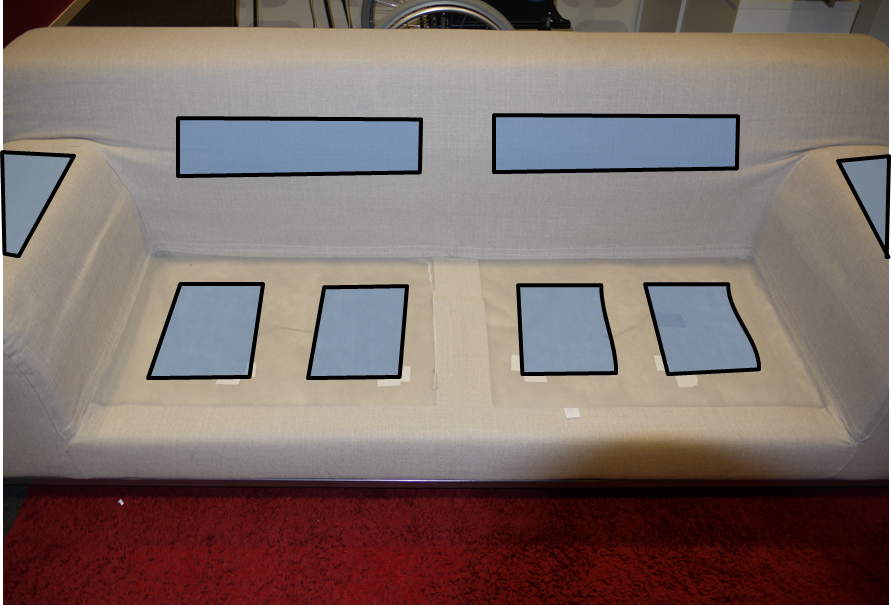
\includegraphics[width=0.7\textwidth]{images/couch_electrodes.png} 
\caption{Electrode placement below upholstery (adapted from \cite{Couch2011})}
\label{fig:couch_electrodes}
\end{figure}
The resulting electrode placement can be seen in Figure \ref{fig:couch_electrodes}. The layout was designed under the additional constriction of using a single sensor kit, supporting up to eight electrodes. Regarding placement it is most important to distinguish two persons and different sitting positions, thus four electrodes are placed below the sitting area. In the back there are two electrodes spread over the entire width to determine the presence of the upper body close to the backrest. The electrodes in the armrests determine a head and are primarily suitable for detecting lying positions. In consequence this setup is suitable for detecting multiple sitting persons, infer information about their sitting position and recognize lying persons. Regarding those postures it showed good results in the prototype's evaluation \cite{Couch2011}.
 
A third and final example for the rationale of electrode placement is the TileTrack system by Valtonen et al, a capacitive person tracking system using floor tiles \cite{Valtonen2009a}. It is a transmit mode system that has the transmitting electrodes placed below the floor tiles and the receiving electrodes are placed in the walls of the area. The main goal of the system is the tracking of persons on the surface. Thus the floor area should be mostly covered by electrodes to establish a good transmission link to the bodies. The receiving electrodes should be able to pick up all signals generated by the body. Valtonen et al. picked wire or plate electrodes that went from floor level to a height of 190cm that covers most typical body sizes. While the system has some shortcomings with regard to applicability in larger rooms, the design rationale is appropriate for narrow rooms or when only movement close to walls has to be detected and had a good precision in their evaluation. Another proposed extension was using receiving electrodes placed in furniture, to provide better resolution in living environments.

\subsection{Data processing}
\begin{figure}[h]
\centering
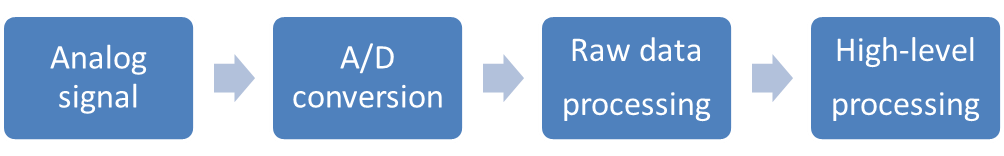
\includegraphics[width=0.8\textwidth]{images/proc_pipe}
\caption{Abstracted sensor data processing pipeline}
\label{fig:rel_proc_pipe}
\end{figure} 
%Figure 10 Abstracted sensor data processing pipeline
In order to acquire usable data from any digital sensor an analog signal has to be acquired and processed. A simplified typical processing pipeline for this is shown in Figure \ref{fig:rel_proc_pipe}. This basic structure is also applicable to the processing of capacitive proximity sensor data. The analog signal is the capacitance of an electric circuit that can be digitized using different methods, e.g. by using the quantized discharge time of the circuit. In the following section some typical steps of raw data processing and high-level processing for capacitive proximity sensors are presented and discussed.
 
\subsubsection{Raw data processing}
Raw data processing of capacitive proximity sensor data is primarily intended to compensate for sensor noise and environmental influences. Noise is an inherent property of any measurement system and describes random unwanted data that is added to a signal. Environmental parameters can have strong influence on the signal of a capacitive sensor system. These effecting factors include temperature, humidity, composition of the air, or grounded objects in close proximity. There are numerous additional preprocessing steps that can be taken, such as different multiplexing methods that may be required in some hardware settings, or signal quantization that reduces the outgoing data to a distinct set of values in order to simplify post processing of different applications. 

\paragraph{Noise Reduction}
In order to deal with noise, some sort of filtering is typically applied. Filtering describes a set of methods that attenuate the parts of a signal that are relevant in a given application. In capacitive proximity sensing we are dealing mostly with high-frequency noise that is added to the signal. Therefore, low-pass filtering can be used to deal with this influence. The most typical examples are average filters that take various samples and calculate an average value, and median filters that are sorting a set of samples and select the median element. Each of those filters has a plethora of potential adaptations that are not too specific to discuss in this limited space. Some adaptations are discussed in the specific prototype sections.
\begin{table}[htbp]
  \centering
  \caption{Baseline calibrations terms and methods}
    \begin{tabular}{lp{6cm}p{5cm}}
    \toprule
    \textbf{Name} & \textbf{Description} & \textbf{Application} \\
    \midrule
    \textbf{Initial calibration} & First set-up of baseline at system start, e.g. by taking the average over various samples & Required for any application \\ \addlinespace
    \textbf{Static baseline} & Baseline that does not change at run-time & For static environments \\ \addlinespace
    \textbf{Dynamic baseline} & Baseline that changes over time & For non-static environments \\ \addlinespace
    \textbf{Drift } & Change of system response to environmental factors at run-time & - \\ \addlinespace
    \textbf{Drift compensation} & Methods to account for occurring drift, by changing the baseline value & Non-static applications \\ \addlinespace
    \textbf{Recalibration} & Change of the baseline value at a specific point in time given a set of rules & Non-static applications \\
    \bottomrule
    \end{tabular}%
  \label{tab:rel_baseline}%
\end{table}%

\paragraph{Baseline Calibration}
A very important aspect of capacitive raw data processing is signal calibration. The generated electric field is subject to changes over time, if either intrinsic parameters change or the environment is modified. Some specific examples include the electronic components heating up, the environmental temperature changing, or objects being moved in and out of detection range. Therefore it is essential to have a well-calibrated and adaptive baseline; that is the sensor signal generated in the environment without the presence of any object that shall be detected. Again, there are numerous methods to adapt and configure the baseline. I have collected a few common terms and methods and give some pointers regarding their application. The results are shown in Table \ref{tab:rel_baseline}. 
\begin{figure}[h]
\centering
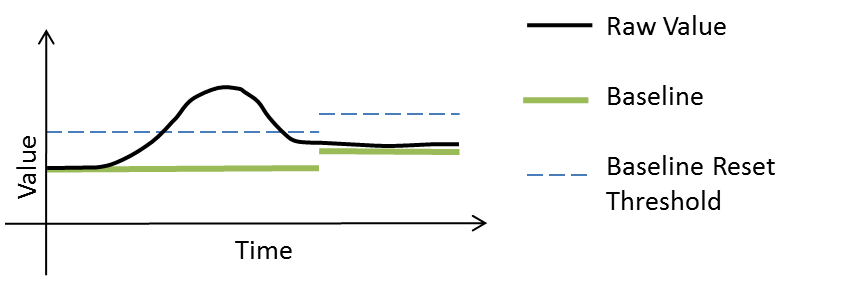
\includegraphics[width=0.5\textwidth]{images/baseline_reset}
\caption{Example of baseline reset using a threshold rule}
\label{fig:rel_base_reset}
\end{figure} 
%Figure 11 Example of baseline reset using a threshold rule
If a dynamic baseline is used, a set of rules will have to be defined that determines at which points in time the baseline has to be recalibrated, what specific methods should be used and the set of parameters that control the methods. One simple example is to define a threshold level that triggers a baseline calibration, as shown in Figure \ref{fig:rel_base_reset}. The raw signal is above the threshold, indicating the presence of a detectable object. Afterwards, it falls back down below the threshold, yet stays for a certain time above the baseline. This triggers a reset of the baseline after a certain amount of time.
\subsubsection{High-level processing}
High-level processing assumes that there are calibrated (and possibly normalized) sensor values that are used in further steps. The goal of any capacitive sensing application is the acquisition of information about a detectable object, e.g. its current position, the material used or the shape. In order to get this information we need to use knowledge about the object and intrinsic properties of the sensor system. In this section I will discuss methods to combine data from various sensors using the system properties, how to track the position of an object using different methods and how to recognize specific features. An overview of the methods in abridged form is given in Table \ref{tab:rel_highlevel}. 
\begin{table}[htbp]
  \centering
  \caption{Overview of high-level processing methods for capacitive proximity sensors}
    \begin{tabular}{lp{5cm}}
    \toprule
    \textbf{Name} & \textbf{Description} \\
    \midrule
    \textbf{Sensor data fusion} & Combining sensor data into a shared representational format \\ \addlinespace
    \textbf{Uniform fusion} & Sensor data fusion that combines all data into a single common format \\ \addlinespace
    \textbf{Heterogeneous fusion} & Sensor data fusion that combines groups of data to serve multiple purposes \\ \addlinespace
    \textbf{Object tracking } & Continuous identification of an object within the systems range \\ \addlinespace
    \textbf{Single object tracking} & Methods to realize object tracking for a single detectable object \\ \addlinespace
    \textbf{Multiple object tracking} & Methods to realize object tracking for multiple objects \\ \addlinespace
    \textbf{Feature recognition} & Identifying certain parameters of an object within the system range \\
    \bottomrule
    \end{tabular}%
  \label{tab:rel_highlevel}
\end{table}%

\paragraph{Sensor data fusion}
Sensor data fusion in its most general terms describes "the theory, techniques and tools which are used for combining sensor data, or data derived from sensory data, into a common representational format" \cite{mitchell2007introduction}. Using the combined information from various capacitive proximity sensors it is posisble to generate high-level information that exceeds the capabilities of a single sensor. Two methods can be  distinguished. The first is uniform fusion that uses the information from all involved sensors in one common way. The second is heterogeneous fusion that combines groups of involved sensors that serve multiple purposes, yet are attached to a single system. A simple example for the latter would be a single large electrode sensor that detects the presence of a hand from a farther distance and then a combination of various small electrodes that track single fingers. 

Sensor data fusion often requires taking into account some additional information we possess about the system. A classic example is the precision or bias of the sensor. Various methods, e.g. the class of Kalman filters, use weighted information from several sensor sources \cite{welch1995introduction}. If we know that a certain sensor is only half as precise as another one working in collaborating, the weighting factors can be adapted accordingly. 

One of the most important additional information that can be used when fusing data of capacitive proximity sensors, is the geometric layout of the system. This describes position and size of all electrodes that are integrated. Using this information is crucial when trying to localize an object. A simple example would be applying a weighted average algorithm on a set of sensors. In order to determine object location relative to the plane a weighted average algorithm is used. The linear object location $\overline{x}$ is calculated using the sums over sensor positions $x_i$ and sensor values $v_i$ as weight:
\begin{equation}
\overline{x}=\frac{\sum^n_{i=1}{v_i x_i}}{\sum^n_{i=1}{v_i}}
\end{equation}
Using similar methods we are able to determine the location of multiple objects or additional dimensions of the position. However, it is possible to use other information in the fusion process as well. The electrode material may result in a different response and thus should be treated differently in a fused data representation and can be weighted. Another example is the shape of the electrode that may result in different responses. How to apply sensor data fusion is strongly depending on the application and the desired common representation that is most suitable for subsequent calculations.

\paragraph{Object tracking}
In the previous section about sensor data fusion I have shortly discussed a method to determine the linear position of a single object using a linear array of capacitive proximity sensor. This is a basic example of a group of methods associated to object tracking. In computer vision applications they can be defined as "the problem of estimating a trajectory of an object in an image plane as it moves around a scene" \cite{yilmaz2006object}. The analogy to capacitive applications is viable if we consider a 3D scene and a distinct interaction space instead of a scene. 

Capacitive proximity sensors allow the detection of conductive objects within their range. However, as this presence is determined indirectly using the influence on an electric field it is not possible to get a direct association between the actual distance between sensor and object and the resulting sensor value. The created electric field is only analytically descriptive for very specific, theoretic classes of objects \cite{Baxter1996}. Nonetheless, we are able to get a relative distance measurement. If we combine this proximity value using geometric information about the electrode location we can infer the relative position of an object in the sensing area. The weighted average method presented in the previous section is one option for relative positioning. Another method is trilateration, similar to many radio-based localization applications, that uses the known location of three or more points and the known distance to the position to be determined. In case of capacitive proximity sensing this position is determined relative to the electrodes as there is no absolute distance measurement. 
A more complex example for direct calculation was presented by Smith, who formulated the issue of detecting multiple objects as a forward problem and used numerical methods to estimate the position and orientation of two hands \cite{smith1999thesis}.
\begin{figure}[h]
\centering
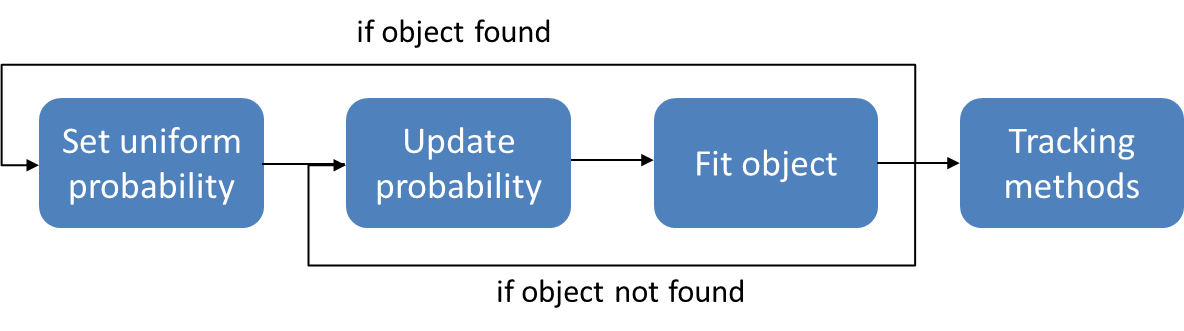
\includegraphics[width=0.7\textwidth]{images/prob_methods}
\caption{Generic pipeline of probability based methods of capacitive proximity sensing}
\label{fig:rel_prob_method}
\end{figure}
%Figure 12 Generic pipeline of probability based methods of capacitive proximity sensing
A second class of methods to track objects is not relying on direct geometrical calculations but instead formulates a numerical solution to a probability distribution. The initial assumption is that the probability of an object to be at a certain point in the detection area is uniform. The methods then follow a few basic steps, as shown in Figure \ref{fig:rel_prob_method}. At first the probability is updated based on the current sensor readings and a priori knowledge about the system. Afterwards it is attempted to fit the objects into the resulting probabilities. This step may or may not work, meaning that it can result in no object found. In the latter case the process will have to start at the beginning. If an object is found the probability update may use the current object location in the update algorithm, thus starting with a non-uniform probability distribution.
One example for probability-based object recognition using capacitive proximity sensors was presented by Grosse-Puppendahl et al. \cite{grosse2013swiss}. Using a model suggested by Smith the basic idea is using the assumption that an object may be present anywhere, remove regions where no objects can be present and then fit an object into the remaining space. This method additionally uses particle filters to track object locations over time. This also allows tracking multiple objects. 

Throughout the years various methods have been suggested for supporting multi-object tracking using capacitive sensors. Touch screens often use inversion of the sender signal to reliably detect the positions of multiple points; however, this method can't be used in proximity applications \cite{wilson2007}. Some of the previously presented methods support the tracking of two or more objects. There are still various limitations, particularly if not only the object location but also various other features such as rotation should be tracked. This is still an area of ongoing research, leading to the next area of high-level processing - feature recognition.
\begin{table}[htbp]
  \centering
  \caption{Feature recognition methods}
    \begin{tabular}{lp{7cm}}
    \toprule
    \textbf{Name} & \textbf{Description} \\
    \midrule
    \textbf{Data-driven  methods} & Directly associate input data to output features using various methods, e.g. machine learning and training data \\ \addlinespace
    \textbf{Model-driven methods} & Input data is manipulating a pre-defined model of the system that is latter mapped to the output \\ \addlinespace
    \textbf{Neural networks} & Computational models using a network of neuron-like objects that are often used in machine learning \\ \addlinespace
    \textbf{Pattern recognition} & Methods that look for certain patterns in a set of input data \\
    \bottomrule
    \end{tabular}%
  \label{tab:rel_feature}%
\end{table}%

\paragraph{Feature recognition}
Feature recognition is primarily used as a term in image processing, traditionally in computer-aided design applications to recognize specific geometric properties of an object but also picture analysis, e.g. in facial recognition \cite{han2000manufacturing,belhumeur1997eigenfaces}. 
In the domain of capacitive proximity sensing, feature recognition can be defined as the acquisition of non-location information from any detectable object. An important feature in industrial applications is the material of an object \cite{Baxter1996}. With regards to recognizing additional features a system was presented by Wimmer et al. - Thracker \cite{Wimmer2006}, a prototype augmenting a regular monitor with capacitive proximity sensors. In addition to recognizing hand position the system is able to detect grasp gestures, which can be used to select items on the screen and perform pick and drop operations. Capacitive sensors can also be used to distinguish between persons and a children's seat on the passenger side of a car \cite{george2009seat}. 
The methods to recognize the features can be divers, ranging from typical machine learning algorithms, to model-based approaches. An incomplete list is given in Table \ref{tab:rel_feature}. In order to keep this work contained I will refrain from a deeper discussion at this point.

